\chapter{研究背景}
\label{chap:webapi}

ユーザーの拡張現実や明晰夢における認識度や要求について事前調査、睡眠中に見る夢の分析を行った。その結果に基づいてDreamtravelerの開発に反映した点について述べる。

\section{拡張現実について調査}
人がどのような拡張現実を望んでいるかを調査するため、理系の学生7人、文系の学生7人、サラリーマン10人、主婦3人を含めた20〜60歳の男女27人にオンラインアンケートをした。これらのインタビュー結果を経て一般的なユーザのニーズを把握し、Dreamtravelerの有効性やDreamtravelerが解決すべき問題について明らかにする。

\subsection{拡張現実を体験するために一般的な人々が支払う金額}
機能性やデザインの詳細を説明した上で、仮想現実を見る手段として次の選択肢から選んでもらった。OCULOUS Rift:85278円、ハコスコ:1500円、iWink:36478円、タカラトミー夢工房:15984円、Dreamtraveler :無料。すると図\ref{userNeedCost}のように、一般的なユーザーの中には拡張現実を体験するためにOCULOUS Riftなどの高額なデバイスを購入しようとする人は少ないということが分かった。ハコスコだと少し数が増えるが、これらのデータから無料で簡単に手に入れることができるツールを多くの人が必要としていることが証明された。

\begin{figure}[htbp]
\begin{center}
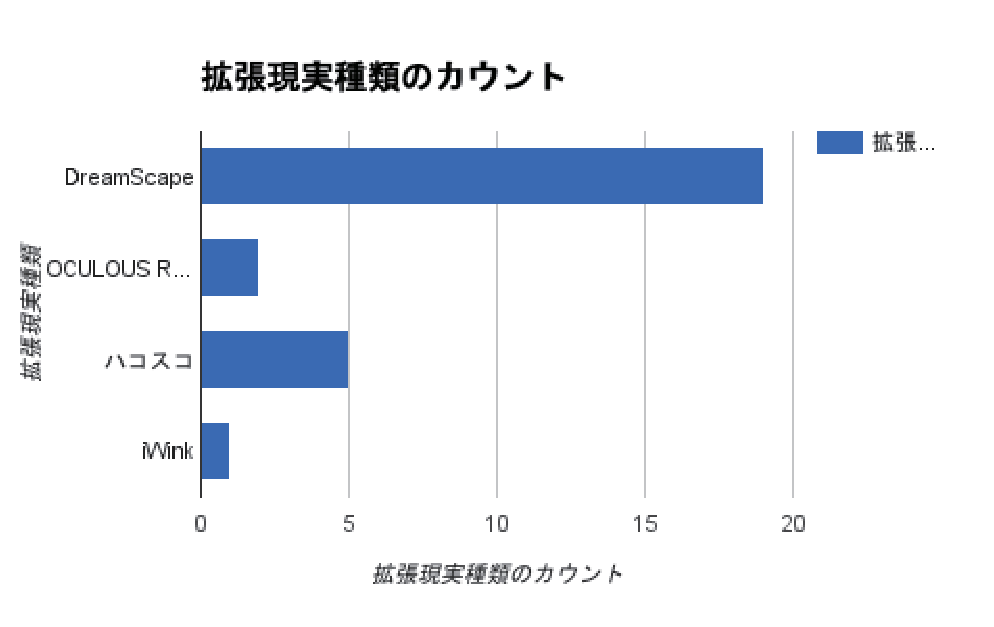
\includegraphics[width=15cm]{eps/VRselection.eps}
\caption{拡張現実を体験するために一般的ユーザーが選ぶ手段}
 \label{userNeedCost}
\end{center}
\end{figure}

\subsection{拡張現実を体験したいタイミング}
拡張現実を体験したいタイミングとして、睡眠中と起きている時間帯でどちらが好ましいかについて調査を行った。すると睡眠中と答えたのは52\%、起床中と答えたのは48\%だった。よって結果にはあまり差がなかった。睡眠中を選択した人は理由として「睡眠時間の有効活用のため」と答えた。比べて起きている時と選択した人は「起きたら忘れてしまうかもしれないから、意識のある時に体験したい」と答えた。よってDreamtravelerの開発において実際に睡眠中の拡張現実がユーザーにどのような体験を与えるかを研究することは意義があると考えられる。


\section{睡眠に関する調査}
\subsection{睡眠段階(睡眠の深さのレベル)と夢}
睡眠は身体を休めるためにある。そして人生の1/3を占める活動である。睡眠中人は2つの睡眠段階、REM睡眠とnonREM睡眠を90分間隔で行き来している\cite{Dement}。REMはRapid Eye Movementの略だ。筑波大と理化学研究所の研究によるとREM睡眠中は記憶形成や脳機能回復の作用がある脳波(デルタ波)が多く見られるというのが通説である\cite{tsukuba}。そしてREM睡眠中は心拍数や眼球の運動が活発化する。REM睡眠の最中に起きたときは夢も比較的覚えている\cite{remNonRem}。一方nonREM睡眠中は脳も身体も休んでいる。\\
 図\ref{SleepHypnogram}は平均的な睡眠のサイクルを示したものである。睡眠に突入して初めてのREM睡眠は10〜12分でもっとも短い。2度目のREM睡眠は15〜20分。最後の夢は15分であるが、通常はアラームなどによって不意に中断されることが多い。平均的に一晩で5〜7回夢をみる。一般的な人生で人は6年間夢を見る。
 夢は環境、時間軸と登場人物がマッチしない場合など、不合理であったり、異様な内容のことが多いが大抵の場合人は夢を見ていることに気がつかない。それは論理的思考力を担う前頭前皮質の機能が低下しているためだ\cite{cortex}。

\begin{figure}[htbp]
\begin{center}
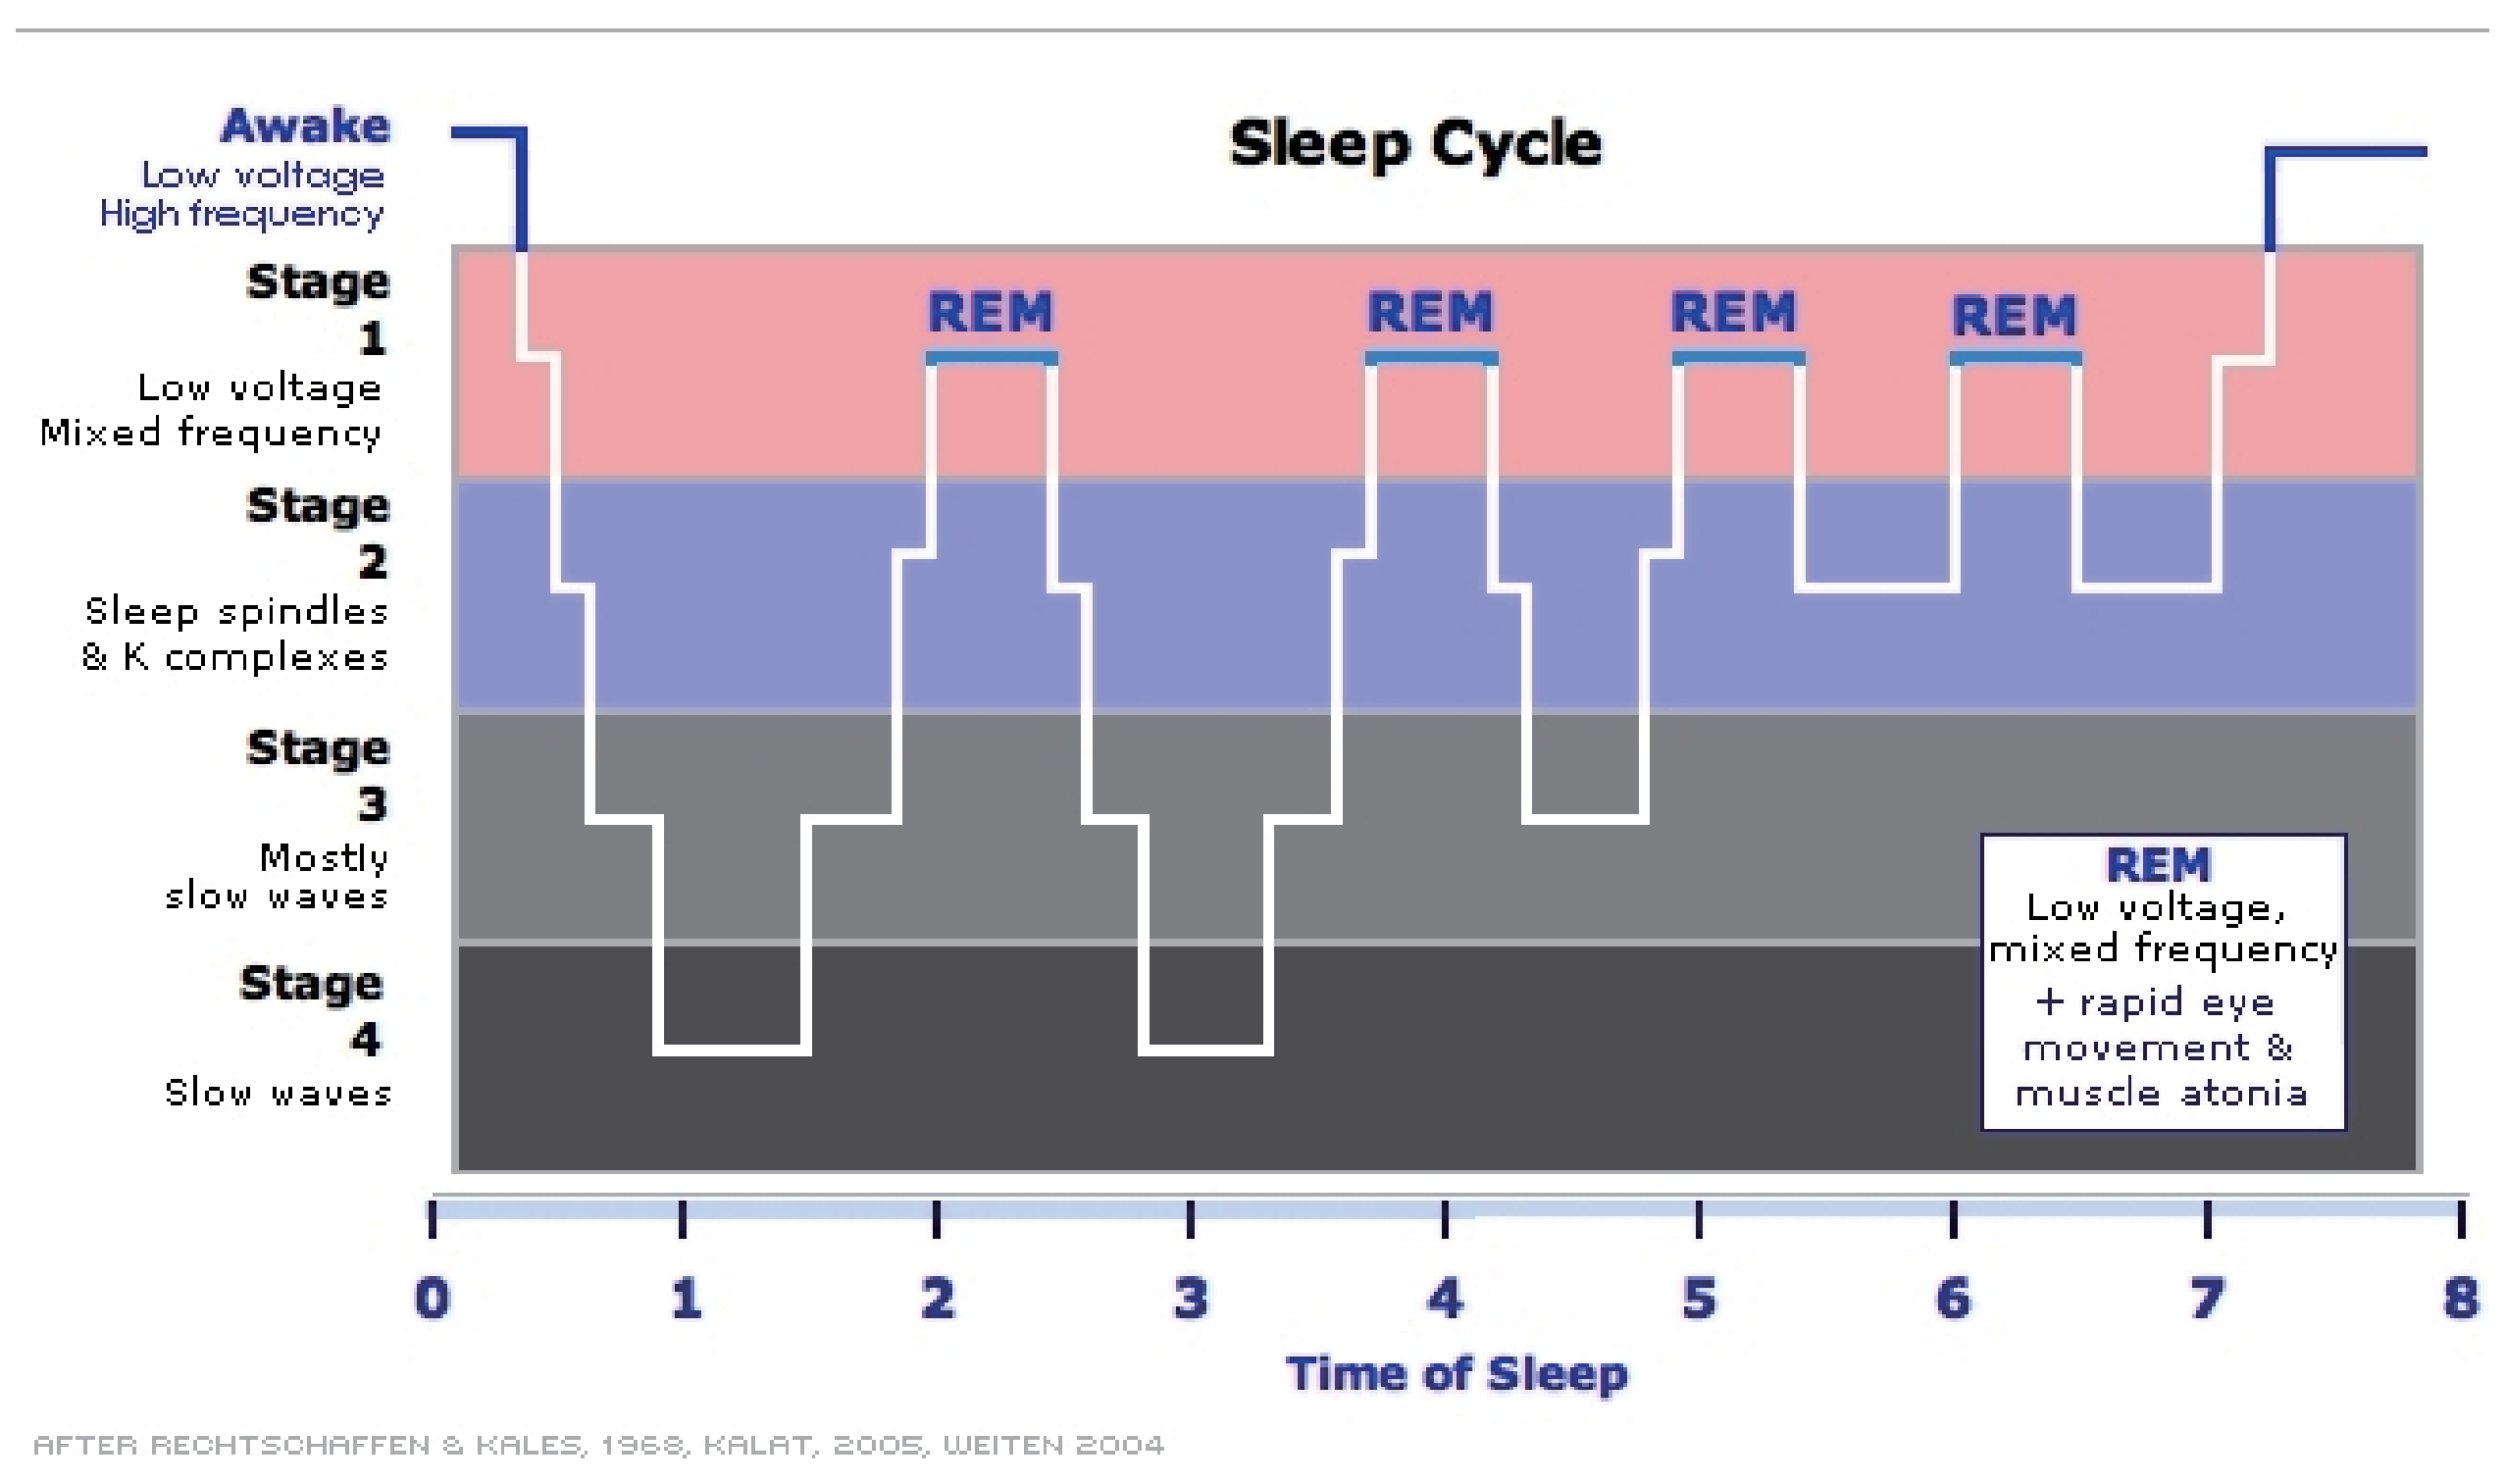
\includegraphics[width=15cm]{eps/SleepHypnogram.eps}
\caption{nonREMとREM睡眠}
\label{SleepHypnogram}
\end{center}
\end{figure}

\subsection{人はなぜ夢を見るのか}
Sigmund Freudによると無意識の欲求や感情、抑圧された子供の頃の記憶、整理的欲求などが影響を与えるという\cite{freud}。Jie Zhangは夢は短期的な記憶を長期的な記憶に変換するためのプロセスであると述べる。具体的には過去の記憶の中で関連性の強い記憶を繋げたり、必要のない記憶を消したりしている\cite{Zhang}。この図\ref{brainZhang}は睡眠中の脳の働きを表す。幼児の平均睡眠時間は16時間でそのう内の50\%をREM睡眠が占める。一方成人の平均睡眠時間は7時間でREM睡眠の長さも短い。年齢が若いほどREM睡眠の周期が長いのは、経験すること全てが新しいため、それだけ多くのことを記憶しなければならないことと、脳の空き容量が多いためと説明されている。

\begin{figure}[htbp]
\begin{center}
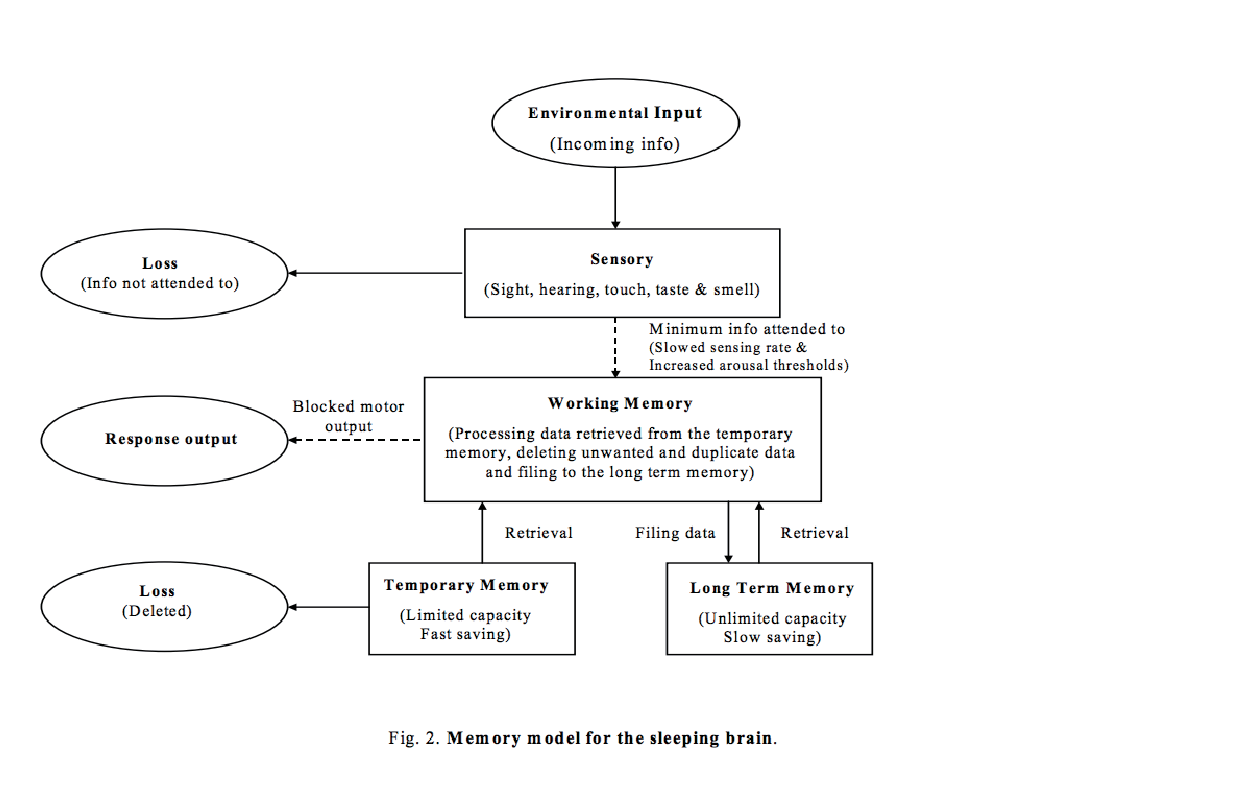
\includegraphics[width=15cm]{eps/sleepBrainModel.eps}
\caption{REM睡眠中の脳の働き睡眠}
\label{brainZhang}
\end{center}
\end{figure}

\subsection{睡眠と寝返りの関係性}
人は睡眠段階を移行させるために寝返りを行う習性があるとされている。要するに睡眠サイクルのスイッチのような働きをする。\cite{negaeri}

\section{明晰夢に関する調査}
\subsection{夢をどのくらい記憶しているか}
夢の操作に成功したとしてもその夢を覚えていなければ意味がない。そこで実験を始める前に一般的に人は夢の内容を起床後どのくらい覚えているのかを調査した。図\ref{rememberDream}がから読み取れるように、夢をよく覚えていると答えた人は少数だった。

\begin{figure}[htbp]
\begin{center}
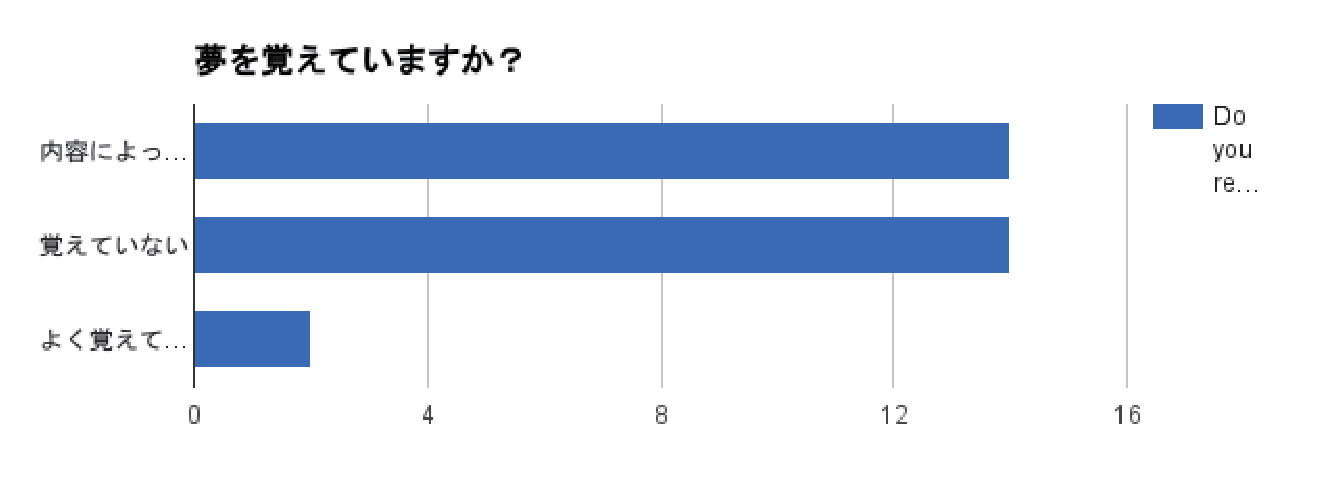
\includegraphics[width=15cm]{eps/remember.eps}
\caption{夢を覚えている比率}
\label{rememberDream}
\end{center}
\end{figure}

覚えている夢は刺激的、怖い夢、繰り返し見た夢というのが多く、日常的な夢は忘れがちであるということが分かった。人は睡眠中の夢の90\%を起床後5分間で忘れるという。Jie ZhangによるとREM睡眠中は短期的な記憶を担っている脳は長期的な記憶への移行に注力していて、インプットの部分があまり機能していないためであると説明する。ただ起きてすぐに、夢日記で夢を記憶すれば覚えていられることが可能なのだ\cite{forgetDreams}。よってDreamtravelerには5分以内に夢の内容を記憶するための日記の機能を加えることに決めた。夢日記は習慣的につけることで効果が出ると言われている。この事実からDreamtravelerの被験者には2週間前から枕の横に紙とペンを置いて起床後すぐに夢の内容を書く習慣を付けてもらうことにした。

\subsection{夢に影響を与えやすい外的刺激}
心理学者フロイトは「夢判断」の中で人は睡眠中の姿勢、環境、身体的刺激によって夢の内容が変化すると述べている\cite{freud}。睡眠中の人間の鼻先を羽毛でくすぐったときに、夢の内容に変化があったことを確認する実験を紹介している。そこで音、体制、匂い、振動、光、などの刺激の中で何が夢に一番影響を与えやすいのかのインタビューで調査をした。以下の図\ref{externalShigeki}がその結果を示す。音が他の刺激よりも影響を与えやすいということが分かった。Dreamtravelerにとって刺激は非常に重要な鍵となるので実験を通してどの刺激が最も有効的なのかを調べた。それについて第3章で述べる。

\begin{figure}[htbp]
\begin{center}
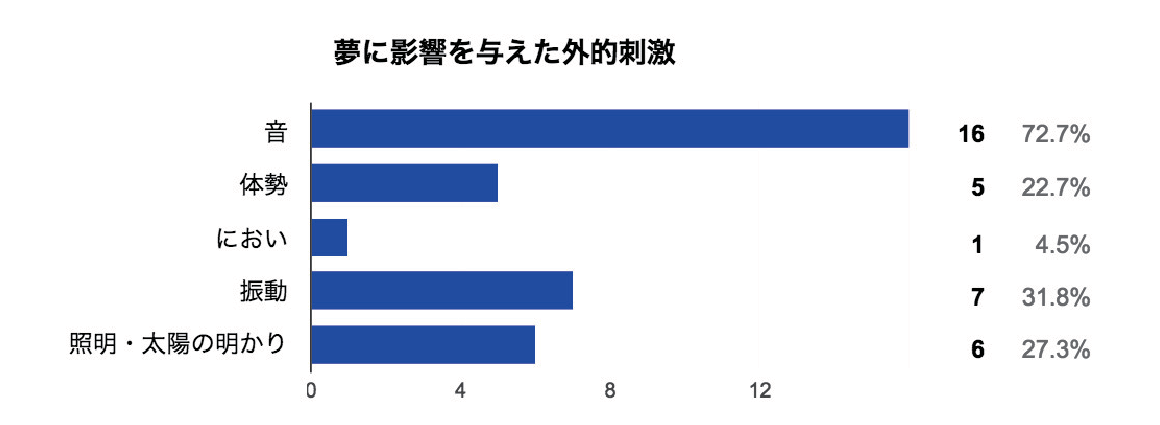
\includegraphics[width=15cm]{eps/input.eps}
\caption{夢に影響を与えた外的刺激}
\label{externalShigeki}
\end{center}
\end{figure}

\subsection{明晰夢のニーズ}
明晰夢を体験したいか否かで質問をしたところ77\%の人が体験したいと答えた。よってDreamtravelerのニーズもあると推測される。

\subsection{明晰夢で体験したい内容}
拡張現実で体験したい内容を調査結果から似ているものをカテゴリー別に分けて、図\ref{desiredDreamTpye}で示した。LOVEタイプ、癒し、元気欲しいタイプ、アドベンチャータイプ、ストーリータイプ、ビジネスタイプとあるがそれぞれの定義を述べる。LOVEタイプとは恋愛や性的行為などが含まれる内容。アドベンチャータイプは冒険など非日常の体験を求める内容。ストリータイプはドラマのように連続性のある夢を求める内容。癒しタイプ・元気欲しいタイプは娯楽を求める内容。原強化タイプは睡眠中になんらかの学習を求める内容だ。LOVEタイプと癒し・元気が欲しいタイプが最も多く、少数派として勉強家タイプがあった。

\begin{figure}[htbp]
\begin{center}
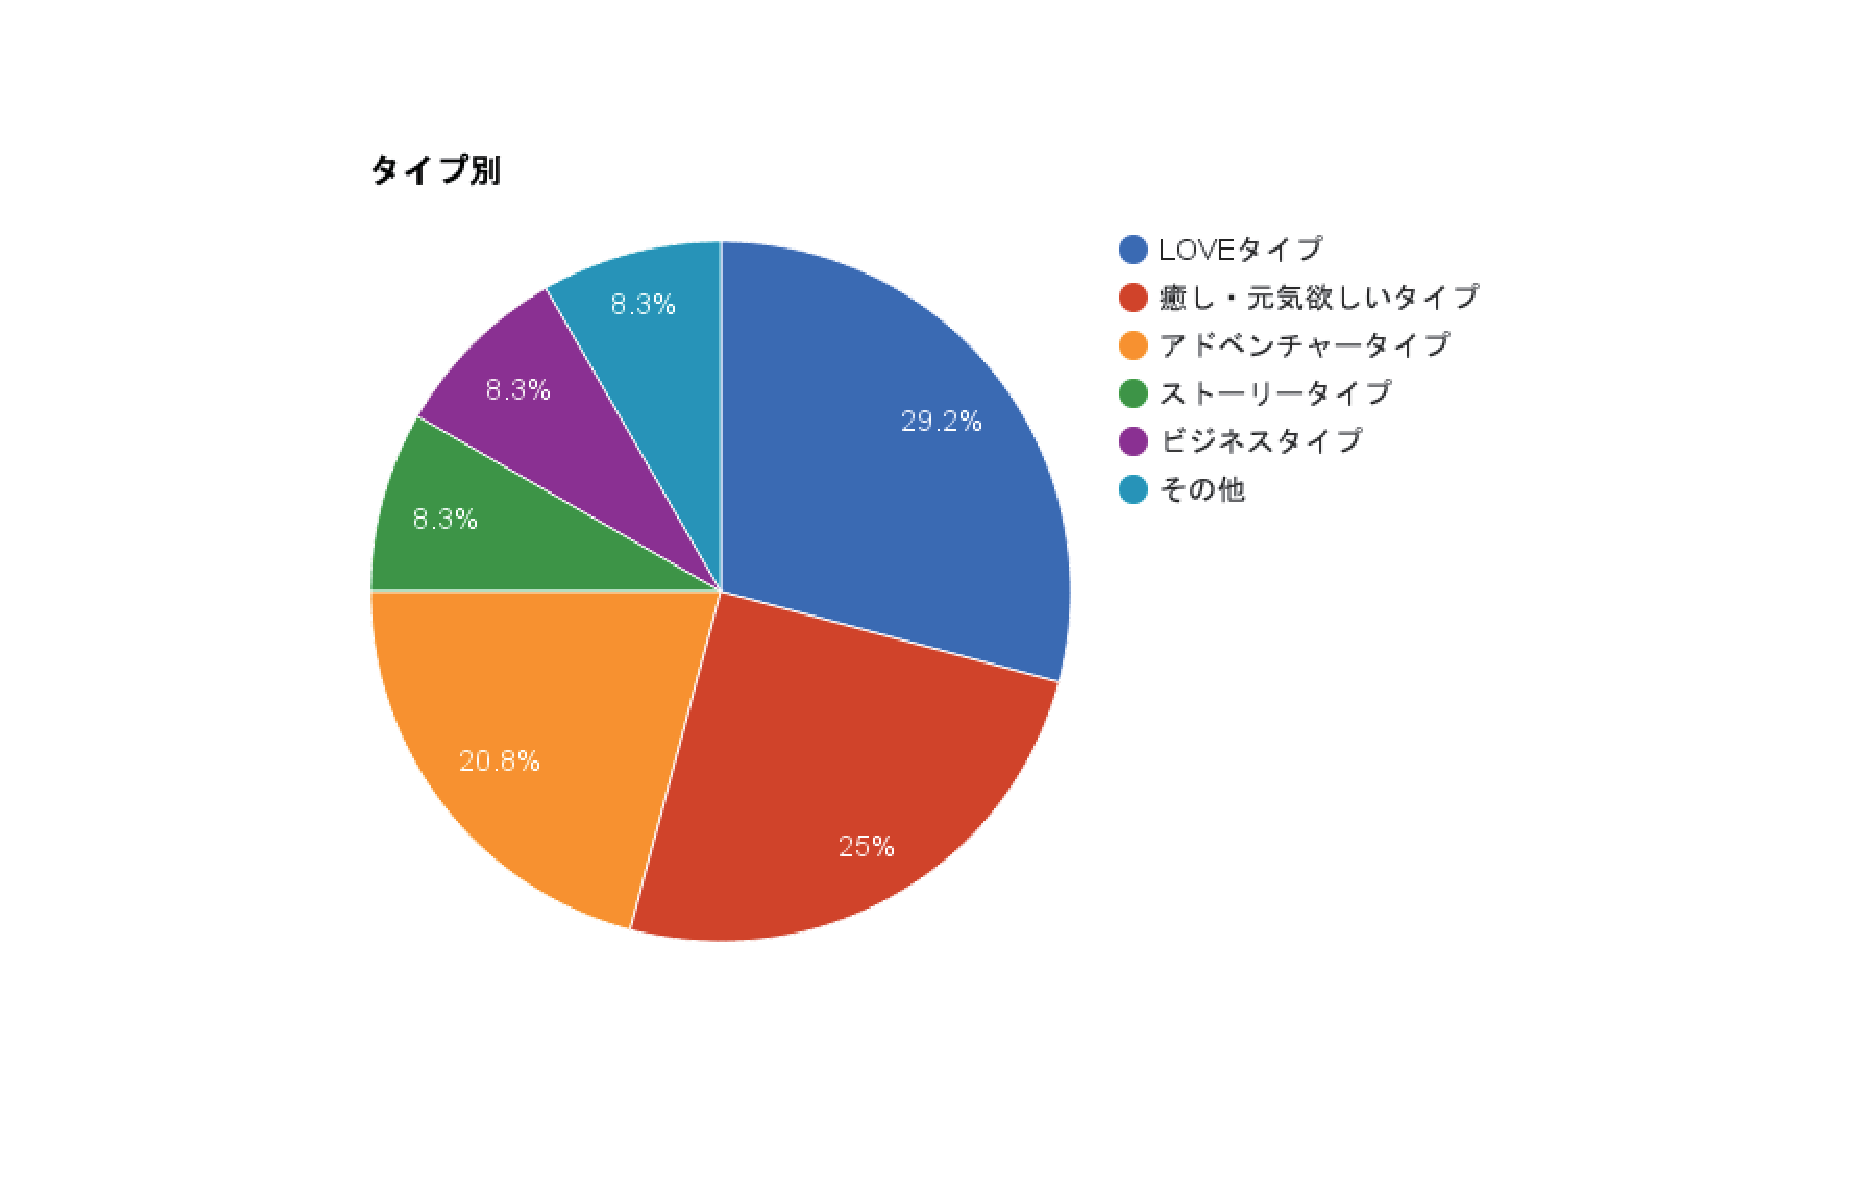
\includegraphics[width=15cm]{eps/dreamType.eps}
\caption{明晰夢で体験したい内容:分析1}
\label{desiredDreamTpye}
\end{center}
\end{figure}

回答をさらに違った方法で分析した結果が\ref{desiredDreamTpye2}である。これらの結果からユーザーによって理想の夢は日常や非日常、具体性や抽象性に隔たりがあり、一貫性が見られないことがわかった。よってDreamtravelerはユーザ一人一人の要望に合った音を選ぶシステムが必要とされることがわかった。

\begin{figure}[htbp]
\begin{center}
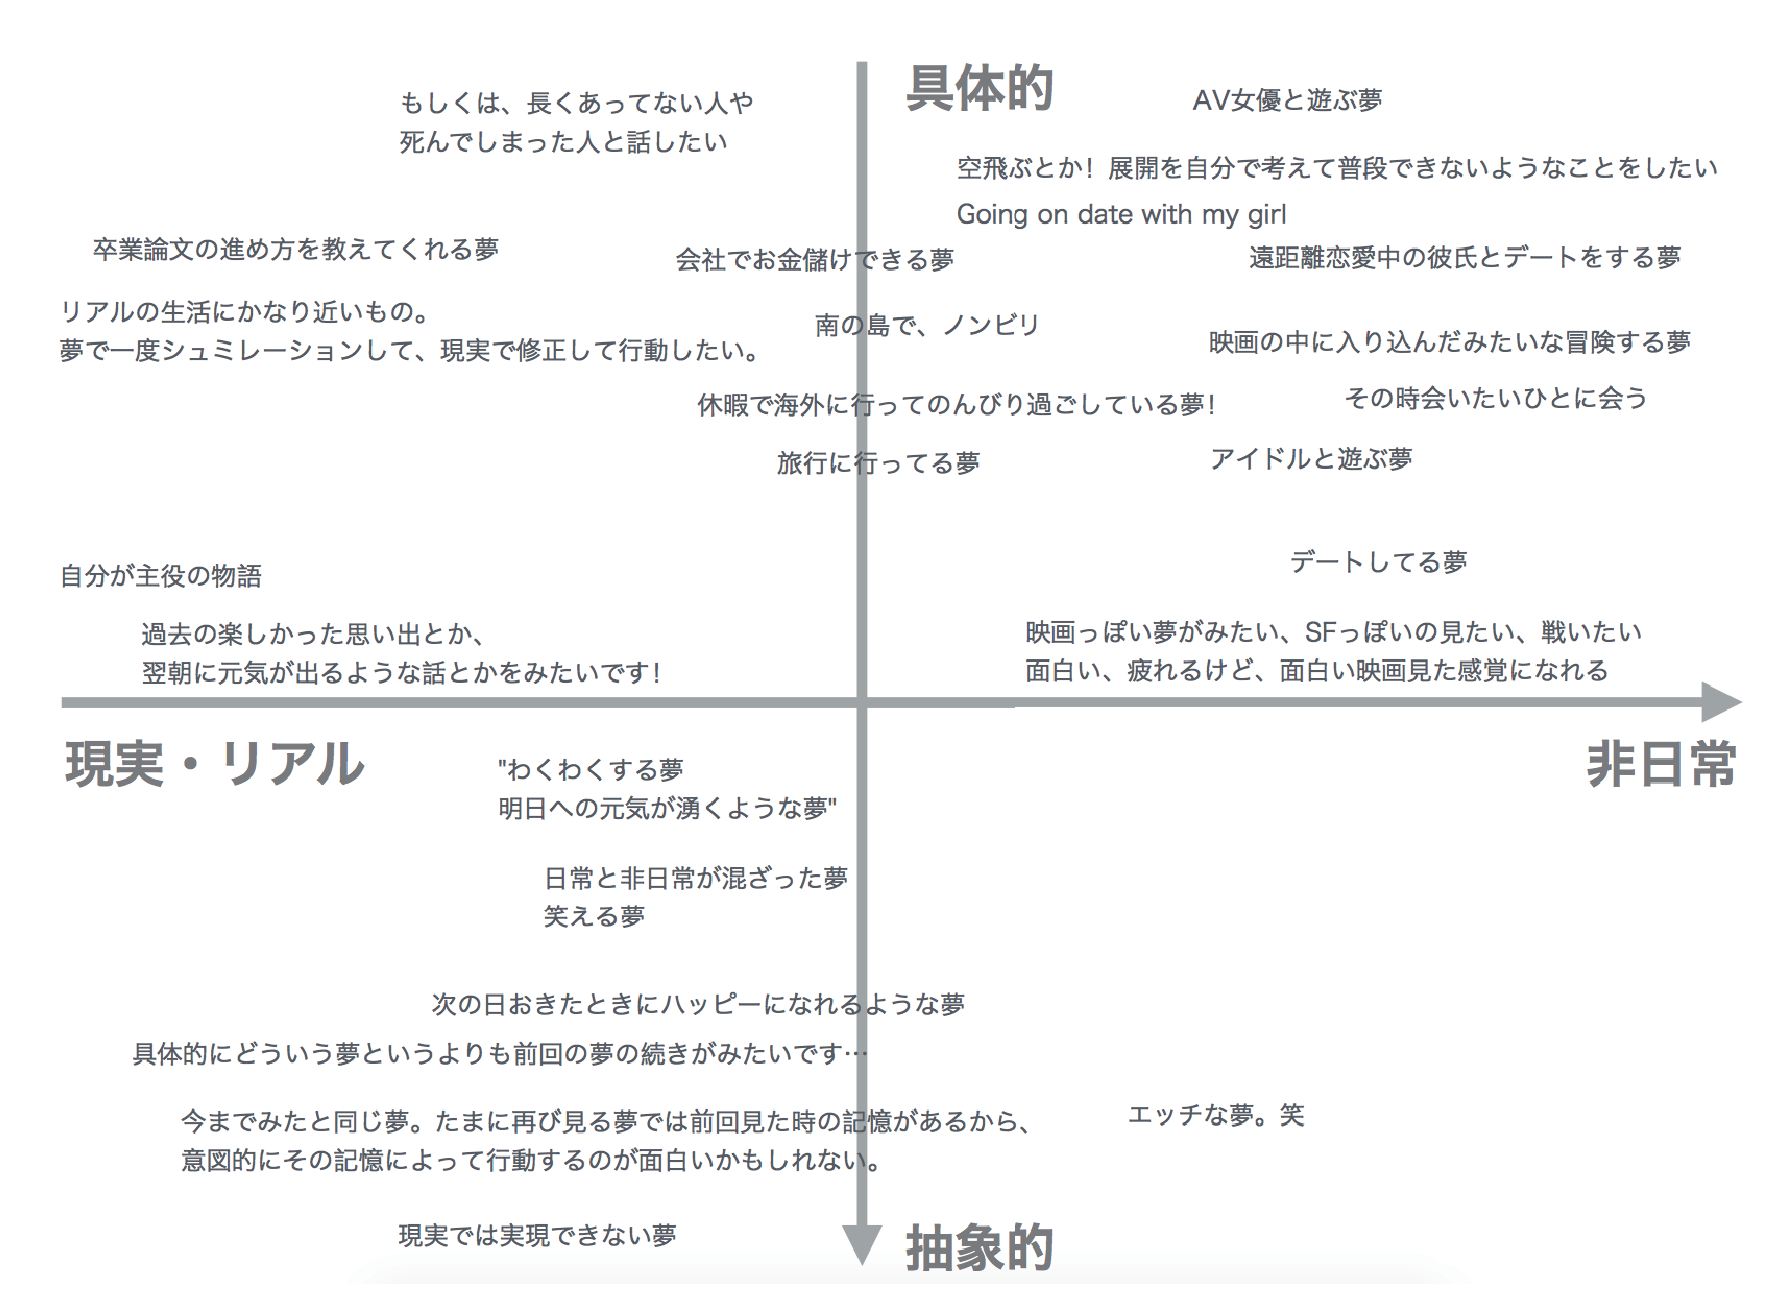
\includegraphics[width=15cm]{eps/whatYouWantToDream.eps}
\caption{明晰夢で体験したい内容:分析2}
\label{desiredDreamTpye2}
\end{center}
\end{figure}

\section{調査から分かったこと}
現実を仮想的に見ることが明晰夢でも可能なのであれば、Dreamtravelerにも興味を示す人が多いということが分かった。明晰夢は睡眠という習慣をより有効に活用し、金銭的コストをかけることなく遂行することができる。求められるのは低価格、高機能、快適なユーザー体験なのでその点に気をつけて開発を進めたい。またコンテンツが見られるようにする対策も必要であろう。